%\subsection{Power Sub-System}
\subsection{Solar Charge Controller}
Solar Chargers are current and voltage regulators that are solar powered themselves. They take in power from PV arrays and deliver optimal power to their electrical load. Due to the overall desired design of our project it has been decided that our own solar charge controller will be built. The heart of our design behind a solar charge controller is a buck boost controller. This takes in a certain voltage range and can be manipulated to output the desired voltage. The power considerations that must be taken into account are the voltage of the micro-controller to be powered as well as the solar power output. The selected micro-controller has an input voltage range of 1.8V to 3.6V with peak performance coming from an input of 3.3v. The selected solar panel has a peak performance output of 6.12v. This means that the proper selection for our buck boost controller must be able to take in a range of voltage around 6v and output a voltage of 3.3v. Once we have the power from the solar panel input into the buck boost controller we will have the proper output to power the load and charge the battery with the remaining power.

\subsection{Batteries}
In this section, we provide an overview of the different types of batteries that we considered for use in our design. These types include lead acid batteries and lithium batteries. We also cover the different characteristics that we considered during the process of choosing a battery type.

\begin{figure}
    \centering
    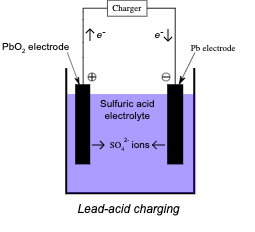
\includegraphics[scale=0.25]{figures/lead-acid-battery.png}
    \caption{The configuration of a lead acid battery.}
    \label{lead-acid-battery} 
\end{figure}

\subsubsection{Lead Acid Batteries}
Lead batteries consist of two electrodes, a negative electrode consisting of lead and a positive electrode consisting of a lead oxide. The two electrodes are submerged in an electrolyte solution comprised of a mixture of water and sulfuric acid. Typically, an electrically insulating material that is chemically permeable is added to ensure the two electrodes do not come into direct contact. The configuration of a lead acid battery can be seen in Figure \ref{lead-acid-battery}, while the chemical equation of the reaction being implemented can be found in Equation \ref{lead-acid-eqn}.

\begin{equation}
    \text{PbO}_2 + \text{Pb} + 2\text{H}_2\text{SO}_4
    \xLeftrightarrow[charge]{discharge}
    2\text{PbSO}_4 + \text{H}_2\text{O}
    \label{lead-acid-eqn}
\end{equation}

\subsubsection{Lithium Batteries}
Lithium batteries differ in a few substantial ways from their lead acid counterparts. The basic component of a lithium battery is a positively charged cathode typically made of a lithium oxide metal that will give off lithium ions. A negatively charged anode that while charging, will store lithium ions from the cathode and while discharging will allow the lithium ions flow through the electrolyte and the electrons through the electrical path back to the cathode. The Electrolyte is usually a material that is highly ionic conductive, this will permit lithium ions to pass through while the electrons will be kept in the anode. The last material is called the separator and it usually consists of polyethylene or polypropylene. The separators' job is to not inhibit the other functions of the battery but also keep the anode and cathode from coming into physical contact. The configuration of a lithium-ion battery can be found in Figure \ref{lithium-ion-battery}.

\begin{figure}
    \centering
    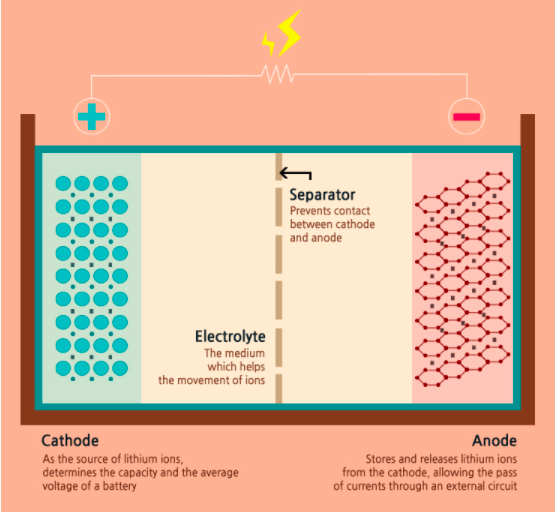
\includegraphics[scale=0.4]{figures/lithium ion battery.png}
    \caption{The configuration of a lithium ion battery.}
    \label{lithium-ion-battery} 
\end{figure}

\subsubsection{Battery Characteristics}
To utterly understand which battery is the right choice for a project one must look at how these methods of constructing a battery will affect the overall characteristics of the battery. The characteristics that impact the usefulness of a battery are as follows: Discharge Curve, Energy Density, Temperature Dependence, Service Life, Charge/Discharge Cycle, and Cost. Once we have amassed information around each characteristic we can then compare Lead acid to lithium batteries more thoroughly. From there if there is not an overall better choice in each and every category we will decide based on which characteristic is most important to complete the objectives of the project. For instance if it is determined that lithium would put us out of our needed price range but is only marginally better than lead acid in other categories then our overall decision will be impacted. Much like any well thought out purchase we must look at each characteristic to gain a better understanding of how our project is being designed and where money is being allocated to.

\paragraph{Discharge Curve}
A discharge curve is a graph that plots Voltage against percentage of the capacity discharged. Essentially the Output voltage of a battery will lower as the battery is used up. Given this effect the most desirable curve would be flat (keeping voltage consistent at every level of discharge), so let us look at the average discharge curve of our lead acid and lithium-ion batteries. Figure \ref{fig:discharge-curve} shows example discharge curves one might find in a lithium ion and lead acid batteries. The figure has been provided by Power Tech, an energy storage system manufacturer. This figure shows first hand how steadily lead acid batteries drop in voltage as the depth of discharge increases. Meanwhile lithium is kept at a steady for the most part until the depth of discharge reaches upwards of 80 percent.

\begin{figure}
    \centering
    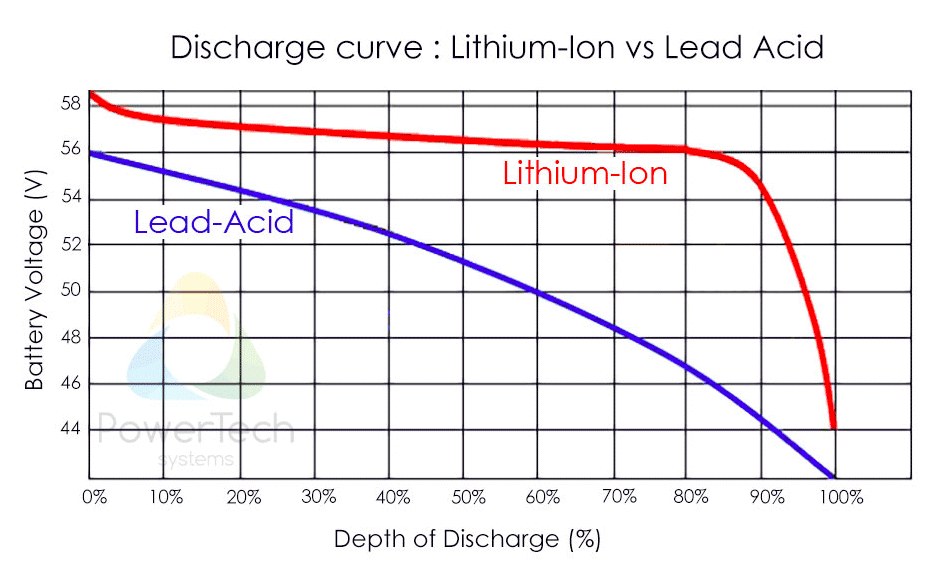
\includegraphics[scale=0.4]{figures/discharge curve.png}
    \caption{A comparison of a lithium ion battery discharge curve and a lead acid battery discharge curve.}
    \label{fig:discharge-curve} 
\end{figure}

\paragraph{Energy Density}
Energy density is the amount of energy you can get out of a battery per unit volume of weight required. Clearly the higher the density the better for a battery. The characteristic known as specific energy density is closely related. However, it considers the Discharge curve of the battery and how it would affect the voltage and current during the battery discharge cycle and is solely measured against weight. An example of the range of energy density and specific energy density can be found in Figure \ref{fig:energy-density} and is provided by the National Aeronautics and Space Administration. This figure shows that lithium far surpasses lead acid in energy density. When it comes to density by volume and density by weight lithium is roughly three times superior to lead acid.

\begin{figure}
    \centering
    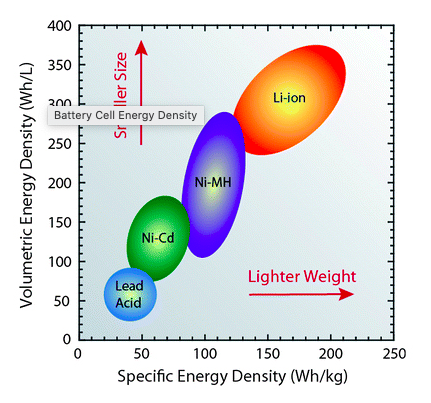
\includegraphics[scale=0.4]{figures/energy density.png}
    \caption{A comparison between volume energy density and specific energy density for various battery types.}
    \label{fig:energy-density} 
\end{figure}

\paragraph{Temperature Dependence}
Battery performance and temperature are highly correlated. Rates of reaction within battery cells themselves are temperature dependent as well as the internal resistance. Low temperatures give higher resistances in a battery, could freeze the electrolyte giving a lower voltage, and cause a steeper discharge curve. At higher temperatures chemicals may decompose or cause enough energy to become available to activate unintended reactions reducing the capacity. The temperature ranges for charging and discharging the viewed battery types are shower in Table (a). 

\paragraph{Service Life}
As each recharge cycle of a rechargeable battery takes place its active components are slowly depleted, lowering its capacity. The industry service life of rechargeable batteries is defined as when the battery's capacity is 80\% of its intended use. The typical service life of rechargeable batteries could be anywhere from 500-1200 cycles. Figure \ref{fig:service-life} shows how repeated cycles influence the types of batteries were researching with the lead acid curve on the left and lithium ion on the right.

\begin{figure}
    \centering
    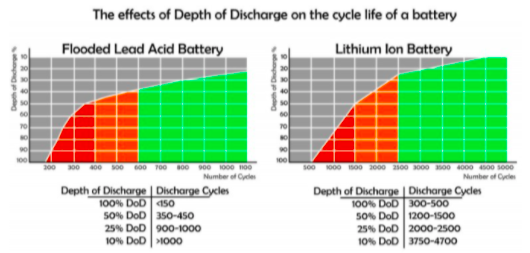
\includegraphics[scale=0.5]{figures/service life.png}
    \caption{A comparison between the service life of lead acid and lithium ion batteries.}
    \label{fig:service-life} 
\end{figure}

\paragraph{Charge Curve}
The charge curve shows the process of charging different batteries. This would include information on the voltage needed to charge, current used to charge, charging times, and capacity of battery. Figure \ref{fig:lead-acid-charge-curve} shows the charge curve for an example lead acid batteries and figure \ref{fig:lithium-charge-curve} shows the charge curve for an example lithium-ion battery. While the charging curves will differ from battery to battery meaning the examples are not completely accurate as to what can be expected the overall structure of the curve will match those with similar chemistry.

\begin{figure}
    \centering
    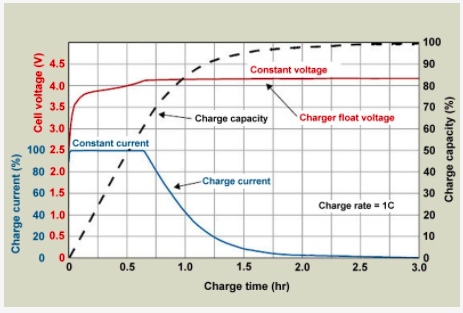
\includegraphics[scale=0.5]{figures/lithium charge curve.png}
    \caption{The charge curve for a lithium ion battery.}
    \label{fig:lithium-charge-curve} 
\end{figure}

\begin{figure}
    \centering
    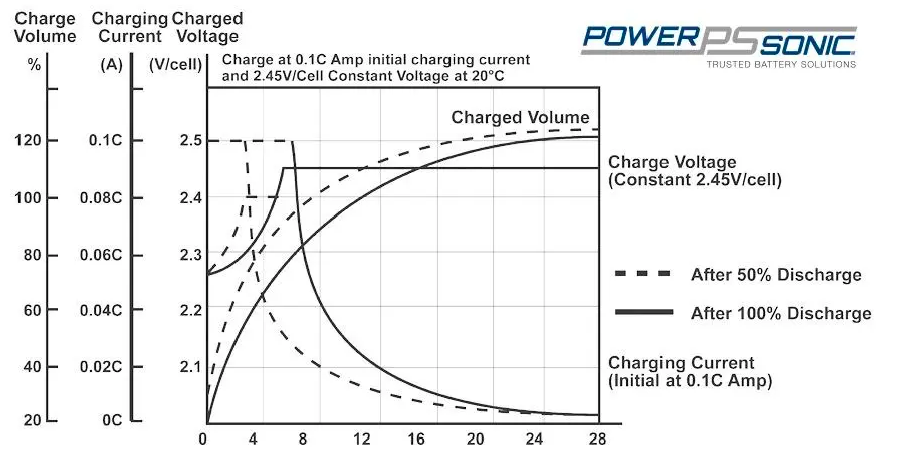
\includegraphics[scale=0.5]{figures/lead acid charge curve.png}
    \caption{The charge curve for a lead acid battery.}
    \label{fig:lead-acid-charge-curve} 
\end{figure}
\paragraph{Cost}
The cost category is self-explanatory. When it comes down to the devices components certain materials can be acquired for a much lower cost than others. For example, according to the US government in 2018 lithium costs \$13,000 per metric ton, while on the other hand during the same year lead hit an all-time high with \$2,600 per metric ton. Table (b) is a handy chart to estimate the cost one could expect to pay for the batteries we have researched. 

\paragraph{Summary}
Within our research many factors of batteries have been observed and noted. Now let's take in our research and decide which battery could best address the needs of this project. 

\paragraph{Decision}
Here is where we will show which battery chemistry, capacity, and amps we will use along with a link to its data sheet. 

\subsection{Solar Panel}

\begin{figure}
    \centering
    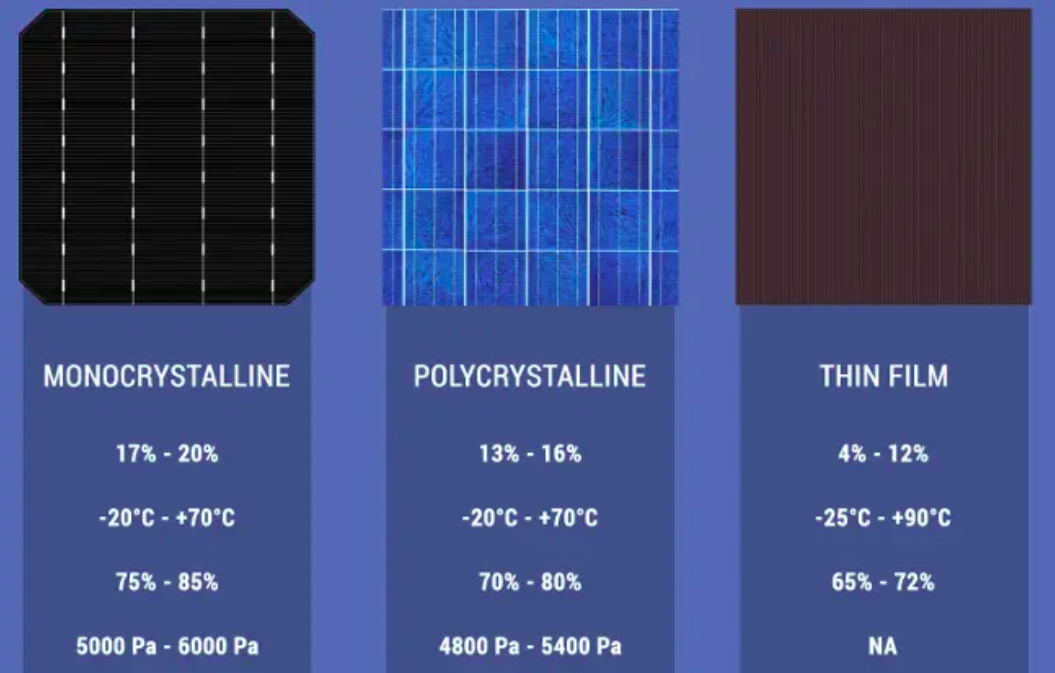
\includegraphics[scale=0.25]{figures/solar panel overview.png}
    \caption{The three types of solar panels.}
    \label{solar-panel-overview} 
\end{figure}

In this section, we will discuss the different types of solar panels that are being considered for use in our design. Discovered in the early 19th century solar panels utilize the photovoltaic effect. This phenomenon was observed when certain materials were produced and electric current when exposed to light. The way this phenomenon is utilized is by using two semiconducting materials. One layer must have depleted electrons and when exposed to sunlight some photons are absorbed by the semiconductor which excites the electrons causing them to jump from one semiconductor layer to another. This jump produces a small electric current which when happens in mass makes a usable power source. The most common material to use in solar panels is silicon which is cut and polished into wafers. Some of these wafers are doped to make an electrical imbalance further helping the process. Finally, electrically conductive strips are attached to the cells to absorb the generated current. 

\subsubsection{Monocrystalline Solar Panels}

Like the name suggests monocrystalline solar panels are made from a single crystal of silicon. Having a single crystal gives electrons more room to flow providing greater efficiency providing more power to the load which is the largest advantage of this type of panel. This, however, is more difficult to create, making it the more expensive option. An example of the features one can expect from a monocrystalline panel can be seen in Figure \ref{solar-panel-overview}. 

\subsubsection{Polycrystalline Solar Panels}

Unlike monocrystalline panels these solar panels are made from many crystals of silicon. This offers much less freedom of movement for electrons which gives a much higher efficiency. This is also simpler to build, meaning that costs are lower, which could be a factor in our decision. An example of the features one can expect from a polycrystalline panel can be seen in Figure (b). 

\subsubsection{Thin Film Solar Panels}

Unlike the previous two types of solar panels, thin film solar panels are mostly not made of silicon. They are made of a mixture of materials mostly cadmium telluride, which is comprised into a thin sheet between two transparent conductive layers that help capture sunlight. Thin film solar panels usually have the lowest efficiency and capacity of all solar panel types however they make up for it in durability and flexibility. The main advantage of this type of solar panel is their low weight, profile, and its ability to adhere to whatever required surface it may need to. Figure (c) shows an example of thin film solar panels. 

\subsubsection{Summary}

Here is where we will show which solar panel, we will use along with a link to its data sheet. 


\subsection{USB Power}
